%% ─── Colours ────────────────────────────────────────────────────────────────
\definecolor{stBlue}{RGB}{25,95,195}
\definecolor{stGreen}{RGB}{18,138,95}
\definecolor{bBlu}{RGB}{218,233,255}
\definecolor{brdBlu}{RGB}{75,138,218}
\definecolor{bGrn}{RGB}{208,243,222}
\definecolor{brdGrn}{RGB}{45,168,118}
\definecolor{bYel}{RGB}{255,248,208}
\definecolor{brdYel}{RGB}{198,168,58}
\definecolor{lgray}{RGB}{158,158,158}
\definecolor{arrB}{RGB}{28,88,208}
\definecolor{colN}{RGB}{28,78,198}
\definecolor{colO}{RGB}{198,38,38}
\definecolor{colCl}{RGB}{28,158,28}
\definecolor{colC}{RGB}{78,78,78}
\definecolor{gCol}{RGB}{68,128,218}
\definecolor{vB}{RGB}{128,168,228}
\definecolor{vO}{RGB}{218,158,68}
\definecolor{vG}{RGB}{118,188,128}
\definecolor{vP}{RGB}{158,108,208}
\definecolor{vK}{RGB}{218,108,158}
\definecolor{vC}{RGB}{78,188,198}
\definecolor{s1c}{RGB}{55,118,218}
\definecolor{s2c}{RGB}{218,148,48}
\definecolor{s3c}{RGB}{48,168,98}
\definecolor{s4c}{RGB}{138,58,208}
\definecolor{s5c}{RGB}{208,58,128}
\definecolor{s6c}{RGB}{28,173,193}
\definecolor{s7c}{RGB}{198,138,58}
\definecolor{s8c}{RGB}{78,178,98}
\definecolor{hFill}{RGB}{222,222,222}

\tikzset{
  aC/.style={circle,draw=colC,fill=white,minimum size=10pt,inner sep=0pt,font=\tiny\bfseries,text=colC},
  aN/.style={circle,draw=colN,fill=colN!15,minimum size=10pt,inner sep=0pt,font=\tiny\bfseries,text=colN},
  aO/.style={circle,draw=colO,fill=colO!15,minimum size=10pt,inner sep=0pt,font=\tiny\bfseries,text=colO},
  aCl/.style={circle,draw=colCl,fill=colCl!15,minimum size=11pt,inner sep=0pt,font=\tiny\bfseries,text=colCl},
  gn/.style={circle,draw=gCol!80,fill=gCol!30,minimum size=4pt,inner sep=0pt},
  sn/.style={circle,draw=#1,fill=white,line width=1.3pt,minimum size=22pt,inner sep=0pt,font=\small\bfseries},
  hb/.style={draw=lgray,fill=hFill,minimum width=18pt,minimum height=14pt,inner sep=2pt,font=\small\bfseries},
  evB/.style={draw=vB!80,fill=vB!35,minimum width=#1,minimum height=5pt,inner sep=0pt},
  evO/.style={draw=vO!80,fill=vO!35,minimum width=#1,minimum height=5pt,inner sep=0pt},
  evG/.style={draw=vG!80,fill=vG!35,minimum width=#1,minimum height=5pt,inner sep=0pt},
  evP/.style={draw=vP!80,fill=vP!35,minimum width=#1,minimum height=5pt,inner sep=0pt},
  evK/.style={draw=vK!80,fill=vK!35,minimum width=#1,minimum height=5pt,inner sep=0pt},
  evC/.style={draw=vC!80,fill=vC!35,minimum width=#1,minimum height=5pt,inner sep=0pt},
  sa/.style={->,>=stealth,line width=0.9pt,color=black!75},
  dl/.style={dashed,line width=0.42pt,color=black!18},
  dt/.style={dashed,line width=0.9pt,color=lgray}
}

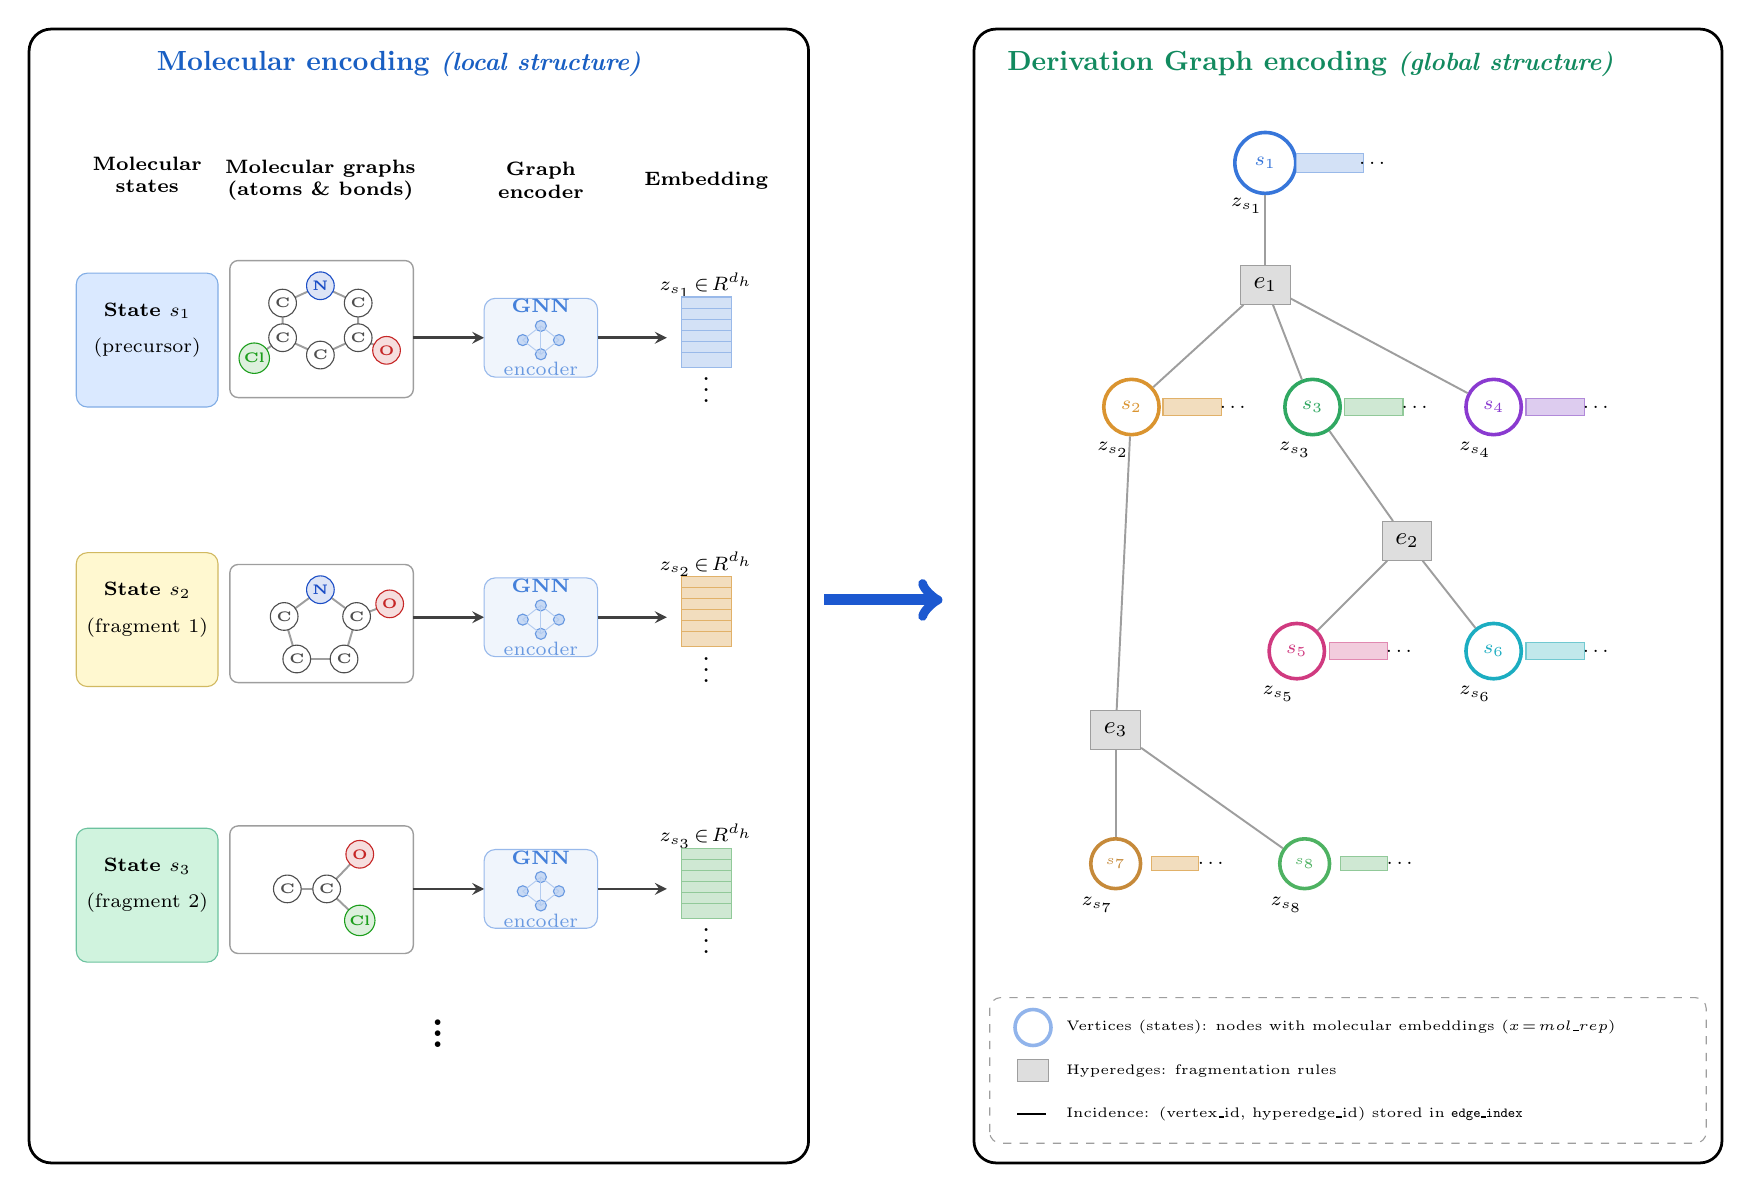
\begin{tikzpicture}[font=\small]

%%──────────────────── STAGE 1 BOX ───────────────────────────────────────────
\draw[rounded corners=8pt,line width=1pt]
  (-0.5,-15.1) rectangle (9.4,-0.7);

\node[anchor=west,font=\normalsize\bfseries,text=stBlue] at (1,-1.15)
  {Molecular encoding \textit{\small(local structure)}};

%% col headers
\node[font=\scriptsize\bfseries,align=center] at (1.0,-2.55)
  {Molecular\\states};
\node[font=\scriptsize\bfseries,align=center] at (3.2,-2.62)
  {Molecular graphs\\(atoms \& bonds)};
\node[font=\scriptsize\bfseries,align=center] at (6.0,-2.62)
  {Graph\\encoder};
\node[font=\scriptsize\bfseries,align=center] at (8.1,-2.62)
  {Embedding};

%%══ ROW 1 – s1 ══════════════════════════════════════════════════════════════
\draw[draw=brdBlu!70,fill=bBlu,rounded corners=4pt]
  (0.1,-3.8) rectangle (1.9,-5.5);
\node[font=\scriptsize\bfseries] at (1.0,-4.28) {State $s_1$};
\node[font=\scriptsize] at (1.0,-4.75) {(precursor)};

%% mol graph s1: 6-ring + O + Cl
\draw[colC!55,line width=0.7pt]
  (2.72,-4.62)--(3.2,-4.84)--(3.68,-4.62)--(3.68,-4.18)--(3.2,-3.96)--(2.72,-4.18)--cycle;
\draw[colC!55,line width=0.7pt] (3.68,-4.62)--(4.04,-4.78);
\draw[colC!55,line width=0.7pt] (2.72,-4.62)--(2.36,-4.88);
\node[aC] at (2.72,-4.62) {C};
\node[aC] at (3.2,-4.84)  {C};
\node[aC] at (3.68,-4.62) {C};
\node[aC] at (3.68,-4.18) {C};
\node[aN] at (3.2,-3.96)  {N};
\node[aC] at (2.72,-4.18) {C};
\node[aO] at (4.04,-4.78) {O};
\node[aCl]at (2.36,-4.88) {Cl};
\draw[lgray,rounded corners=3pt,line width=0.5pt]
  (2.05,-5.38) rectangle (4.38,-3.64);

\draw[sa] (4.38,-4.62)--(5.28,-4.62);
\draw[draw=gCol!55,fill=gCol!8,rounded corners=4pt]
  (5.28,-5.12) rectangle (6.72,-4.12);
\node[font=\scriptsize\bfseries,text=gCol] at (6.0,-4.22) {GNN};
\node[font=\scriptsize,text=gCol!80] at (6.0,-5.02) {encoder};
\foreach \ang in {90,0,270,180}
  \node[gn] at ({6.0+0.23*cos(\ang)},{-4.65+0.18*sin(\ang)}) {};
\foreach \a/\b in {90/0,0/270,270/180,180/90,90/270}
  \draw[gCol!40,line width=0.35pt]
    ({6.0+0.23*cos(\a)},{-4.65+0.18*sin(\a)}) --
    ({6.0+0.23*cos(\b)},{-4.65+0.18*sin(\b)});
\draw[sa] (6.72,-4.62)--(7.6,-4.62);

\node[font=\scriptsize] at (8.1,-3.95) {$z_{s_1}\!\in\!\mathbb{R}^{d_h}$};
\foreach \yy in {-4.2,-4.34,-4.48,-4.62,-4.76,-4.9}
  \node[evB=18pt,minimum height=5.5pt] at (8.1,\yy) {};
\node[font=\normalsize] at (8.1,-5.18) {$\vdots$};

%%══ ROW 2 – s2 ══════════════════════════════════════════════════════════════
\draw[draw=brdYel!80,fill=bYel,rounded corners=4pt]
  (0.1,-7.35) rectangle (1.9,-9.05);
\node[font=\scriptsize\bfseries] at (1.0,-7.83) {State $s_2$};
\node[font=\scriptsize] at (1.0,-8.3) {(fragment 1)};

%% mol graph s2: 5-ring + O
\draw[colC!55,line width=0.7pt]
  (3.2,-7.82)--(2.74,-8.16)--(2.9,-8.7)--(3.5,-8.7)--(3.66,-8.16)--cycle;
\draw[colC!55,line width=0.7pt] (3.66,-8.16)--(4.08,-8.0);
\node[aN] at (3.2,-7.82)  {N};
\node[aC] at (2.74,-8.16) {C};
\node[aC] at (2.9,-8.7)   {C};
\node[aC] at (3.5,-8.7)   {C};
\node[aC] at (3.66,-8.16) {C};
\node[aO] at (4.08,-8.0)  {O};
\draw[lgray,rounded corners=3pt,line width=0.5pt]
  (2.05,-9.0) rectangle (4.38,-7.5);

\draw[sa] (4.38,-8.17)--(5.28,-8.17);
\draw[draw=gCol!55,fill=gCol!8,rounded corners=4pt]
  (5.28,-8.67) rectangle (6.72,-7.67);
\node[font=\scriptsize\bfseries,text=gCol] at (6.0,-7.77) {GNN};
\node[font=\scriptsize,text=gCol!80] at (6.0,-8.57) {encoder};
\foreach \ang in {90,0,270,180}
  \node[gn] at ({6.0+0.23*cos(\ang)},{-8.2+0.18*sin(\ang)}) {};
\foreach \a/\b in {90/0,0/270,270/180,180/90,90/270}
  \draw[gCol!40,line width=0.35pt]
    ({6.0+0.23*cos(\a)},{-8.2+0.18*sin(\a)}) --
    ({6.0+0.23*cos(\b)},{-8.2+0.18*sin(\b)});
\draw[sa] (6.72,-8.17)--(7.6,-8.17);

\node[font=\scriptsize] at (8.1,-7.5) {$z_{s_2}\!\in\!\mathbb{R}^{d_h}$};
\foreach \yy in {-7.75,-7.89,-8.03,-8.17,-8.31,-8.45}
  \node[evO=18pt,minimum height=5.5pt] at (8.1,\yy) {};
\node[font=\normalsize] at (8.1,-8.73) {$\vdots$};

%%══ ROW 3 – s3 ══════════════════════════════════════════════════════════════
\draw[draw=brdGrn!70,fill=bGrn,rounded corners=4pt]
  (0.1,-10.85) rectangle (1.9,-12.55);
\node[font=\scriptsize\bfseries] at (1.0,-11.33) {State $s_3$};
\node[font=\scriptsize] at (1.0,-11.8) {(fragment 2)};

%% mol graph s3
\draw[colC!55,line width=0.7pt] (2.78,-11.62)--(3.28,-11.62);
\draw[colC!55,line width=0.7pt] (3.28,-11.62)--(3.7,-11.18);
\draw[colC!55,line width=0.7pt] (3.28,-11.62)--(3.7,-12.02);
\node[aC]  at (2.78,-11.62) {C};
\node[aC]  at (3.28,-11.62) {C};
\node[aO]  at (3.7,-11.18)  {O};
\node[aCl] at (3.7,-12.02)  {Cl};
\draw[lgray,rounded corners=3pt,line width=0.5pt]
  (2.05,-12.44) rectangle (4.38,-10.82);

\draw[sa] (4.38,-11.62)--(5.28,-11.62);
\draw[draw=gCol!55,fill=gCol!8,rounded corners=4pt]
  (5.28,-12.12) rectangle (6.72,-11.12);
\node[font=\scriptsize\bfseries,text=gCol] at (6.0,-11.22) {GNN};
\node[font=\scriptsize,text=gCol!80] at (6.0,-12.02) {encoder};
\foreach \ang in {90,0,270,180}
  \node[gn] at ({6.0+0.23*cos(\ang)},{-11.65+0.18*sin(\ang)}) {};
\foreach \a/\b in {90/0,0/270,270/180,180/90,90/270}
  \draw[gCol!40,line width=0.35pt]
    ({6.0+0.23*cos(\a)},{-11.65+0.18*sin(\a)}) --
    ({6.0+0.23*cos(\b)},{-11.65+0.18*sin(\b)});
\draw[sa] (6.72,-11.62)--(7.6,-11.62);

\node[font=\scriptsize] at (8.1,-10.95) {$z_{s_3}\!\in\!\mathbb{R}^{d_h}$};
\foreach \yy in {-11.2,-11.34,-11.48,-11.62,-11.76,-11.9}
  \node[evG=18pt,minimum height=5.5pt] at (8.1,\yy) {};
\node[font=\normalsize] at (8.1,-12.18) {$\vdots$};

%% Ellipsis
\node[font=\fontsize{40}{40}\selectfont] at (4.7,-13.35) {$\vdots$};

%%──────────────────── LARGE BLUE ARROW ──────────────────────────────────────
\draw[->, line width=4pt, arrB](9.6,-7.95) -- (11.1,-7.95);

%%──────────────────── STAGE 2 BOX ───────────────────────────────────────────
\draw[rounded corners=8pt,line width=1pt]
  (11.5,-15.1) rectangle (21,-0.7);

\node[anchor=west,font=\normalsize\bfseries,text=stGreen] at (11.8,-1.15)
  {Derivation Graph encoding \textit{\small(global structure)}};

%% s1
\node[sn=s1c,minimum size=22pt] (hs1) at (15.2,-2.4) {};
\node[font=\scriptsize\bfseries,text=s1c] at (15.2,-2.4) {$s_1$};
\node[evB=24pt,minimum height=7pt] at (16.02,-2.4) {};
\node[font=\scriptsize] at (16.58,-2.4) {\ldots};
\node[font=\scriptsize,anchor=north] at (14.97,-2.72) {$z_{s_1}$};

%% s2 s3 s4 row
\node[sn=s2c,minimum size=20pt] (hs2) at (13.5,-5.5) {};
\node[font=\scriptsize\bfseries,text=s2c] at (13.5,-5.5) {$s_2$};
\node[evO=21pt,minimum height=6pt] at (14.27,-5.5) {};
\node[font=\scriptsize] at (14.81,-5.5) {\ldots};
\node[font=\scriptsize,anchor=north] at (13.27,-5.82) {$z_{s_2}$};

\node[sn=s3c,minimum size=20pt] (hs3) at (15.8,-5.5) {};
\node[font=\scriptsize\bfseries,text=s3c] at (15.8,-5.5) {$s_3$};
\node[evG=21pt,minimum height=6pt] at (16.58,-5.5) {};
\node[font=\scriptsize] at (17.12,-5.5) {\ldots};
\node[font=\scriptsize,anchor=north] at (15.58,-5.82) {$z_{s_3}$};

\node[sn=s4c,minimum size=20pt] (hs4) at (18.1,-5.5) {};
\node[font=\scriptsize\bfseries,text=s4c] at (18.1,-5.5) {$s_4$};
\node[evP=21pt,minimum height=6pt] at (18.88,-5.5) {};
\node[font=\scriptsize] at (19.42,-5.5) {\ldots};
\node[font=\scriptsize,anchor=north] at (17.87,-5.82) {$z_{s_4}$};

%% s5 s6 row
\node[sn=s5c,minimum size=20pt] (hs5) at (15.6,-8.6) {};
\node[font=\scriptsize\bfseries,text=s5c] at (15.6,-8.6) {$s_5$};
\node[evK=21pt,minimum height=6pt] at (16.38,-8.6) {};
\node[font=\scriptsize] at (16.92,-8.6) {\ldots};
\node[font=\scriptsize,anchor=north] at (15.37,-8.92) {$z_{s_5}$};

\node[sn=s6c,minimum size=20pt] (hs6) at (18.1,-8.6) {};
\node[font=\scriptsize\bfseries,text=s6c] at (18.1,-8.6) {$s_6$};
\node[evC=21pt,minimum height=6pt] at (18.88,-8.6) {};
\node[font=\scriptsize] at (19.42,-8.6) {\ldots};
\node[font=\scriptsize,anchor=north] at (17.87,-8.92) {$z_{s_6}$};

%% s7 s8 row
\node[sn=s7c,minimum size=18pt] (hs7) at (13.3,-11.3) {};
\node[font=\tiny\bfseries,text=s7c] at (13.3,-11.3) {$s_7$};
\node[evO=17pt,minimum height=5pt] at (14.05,-11.3) {};
\node[font=\scriptsize] at (14.53,-11.3) {\ldots};
\node[font=\scriptsize,anchor=north] at (13.07,-11.6) {$z_{s_7}$};

\node[sn=s8c,minimum size=18pt] (hs8) at (15.7,-11.3) {};
\node[font=\tiny\bfseries,text=s8c] at (15.7,-11.3) {$s_8$};
\node[evG=17pt,minimum height=5pt] at (16.45,-11.3) {};
\node[font=\scriptsize] at (16.93,-11.3) {\ldots};
\node[font=\scriptsize,anchor=north] at (15.47,-11.6) {$z_{s_8}$};

%% e1 incidence node + links to s2 s3 s4
\node[hb] (he1) at (15.2,-3.95) {$e_1$};
\draw[line width=0.7pt,lgray] (hs1)--(he1);
\draw[line width=0.7pt,lgray] (he1)--(hs2);
\draw[line width=0.7pt,lgray] (he1)--(hs3);
\draw[line width=0.7pt,lgray] (he1)--(hs4);

%% e2 incidence node + links s3 s4 → e2 → s5 s6
\node[hb] (he2) at (17.0,-7.2) {$e_2$};
\draw[line width=0.7pt,lgray] (hs3)--(he2);
\draw[line width=0.7pt,lgray] (he2)--(hs5);
\draw[line width=0.7pt,lgray] (he2)--(hs6);

%% e3 incidence node + links s2 → e3 → s7 s8
\node[hb] (he3) at (13.3,-9.6) {$e_3$};
\draw[line width=0.7pt,lgray] (hs2)--(he3);
\draw[line width=0.7pt,lgray] (he3)--(hs7);
\draw[line width=0.7pt,lgray] (he3)--(hs8);

%%──────────────────── LEGEND ─────────────────────────────────────────────────
\draw[draw=lgray,dashed,rounded corners=4pt,fill=white]
  (11.7,-14.85) rectangle (20.8,-13);

\node[sn=s1c!55,minimum size=13pt] at (12.25,-13.38) {};
\node[font=\tiny,align=left,anchor=west] at (12.55,-13.38)
  {Vertices (states): nodes with molecular embeddings ($x\!=\!\text{mol\_rep}$)};

\node[hb,minimum width=11pt,minimum height=8pt] at (12.25,-13.93) {};
\node[font=\tiny,align=left,anchor=west] at (12.55,-13.93)
  {Hyperedges: fragmentation rules};

\draw[line width=0.9pt] (12.05,-14.48)--(12.42,-14.48);
\node[font=\tiny,align=left,anchor=west,text width=7.8cm] at (12.55,-14.48)
  {Incidence: (vertex\_id, hyperedge\_id) stored in \texttt{edge\_index}};

\end{tikzpicture}
